

\documentclass[conference]{IEEEtran}

\usepackage[utf8]{inputenc}
\usepackage[pdftex]{graphicx}
%\usepackage{unicode-math}
%\usepackage{mathtools}
\usepackage{amsmath}


\hyphenation{op-tical net-works semi-conduc-tor}


\begin{document}

\renewcommand{\abstractname}{Resumo}
\renewcommand{\tablename}{TABELA}


\title{Técnica de Visualização Computacional Aplicada a Indicadores de Desenvolvimento Humano de Estados e Cidades do Brasil}


% author names and affiliations
% use a multiple column layout for up to three different
% affiliations
\author{\IEEEauthorblockN{Leandro Ungari Cayres}
\IEEEauthorblockA{Faculdade de Ciências e Tecnologia\\
Universidade Estadual Paulista\\
Presidente Prudente, Brasil\\
\textit{leandroungari@gmail.com}}
}



% make the title area
\maketitle

% As a general rule, do not put math, special symbols or citations
% in the abstract
\begin{abstract}

O Índice de Desenvolvimento Humano busca mensurar o avanço na qualidade de vida de uma população, através de um cálculo matemático que envolve atributos relacionados a educação, saúde e renda. Esse índice tem sido utilizado nas diferentes esferas políticas de governo (municipal, estadual e federal) como apoio a adoção de políticas públicas e investimentos econômicos. A utilização de técnicas de visualização para a interpretação de dados desse contexto, consiste em uma importante ferramenta, pois permite uma apresentação sumarizada dos dados e viabiliza a identificação de padrões em determinadas regiões e a evolução destes conforme uma dada função. Neste trabalho, o processo exploratório foi realizado utilizando a técnica de visualização \textit{Choropleth Map}.

~\\Palavras-chave: Visualização Computacional, Índice de Desenvolvimento Humano e \textit{Choropleth Map}.

\end{abstract}


\IEEEpeerreviewmaketitle


\section{Introdução}
O conceito de Desenvolvimento Humano objetiva mensurar o avanço de uma população não somente considerando os aspectos de âmbito econômico, mas também características sociais, culturais e políticas que influenciam diretamente na qualidade da vida. A partir desse conceito, o Índice de Desenvolvimento Humano (IDH) foi criado com o intuito de contrapor outro indicador muito utilizado, o Produto Interno Bruto (PIB) per capita~\cite{atlas}.

Aos poucos, o IDH tornou-se referência e tem sido utilizado pelos governos federal, estaduais e municipais, sob a denominação de Índice de Desenvolvimento Humano Municipal (IDHM), de forma a apoiar a adoção de políticas públicas e investimentos econômicos para a solução de problemas em contextos sociais específicos.

A utilização de representações visuais para a interpretação dos indicadores consiste em uma importante ferramenta de interpretação, especialmente em um domínio de dados referentes a localidades específicas, possibilita o uso de mapas, e consequentemente, o agrupamento de regiões semelhantes para a identificações de características de uma região em detrimento das demais. 

Dentre as possíveis técnicas de \textit{Visualização Computacional}, para este trabalho foi escolhida a técnica \textit{Choropleth Map} (Mapa Coroplético). Nessa técnica, o conjunto de dados que será visualizado é atribuído a unidades geográficas (bairros, cidades, estados, etc.) sendo representados através do uso de pseudocores.

O presente trabalho está dividido nas seguintes seções: na Seção~\ref{section:fundamento} é apresentado o índice de Desenvolvimento Humano, assim como seu cálculo e os indicadores que o compõem; na Seção~\ref{section:tecnica} é apresentada a técnica de visualização \textit{Choropleth Map}, o histórico e utilização dessa abordagem; a Seção~\ref{section:resultados} é composta pelos estudos de caso executados para avaliação da técnica de visualização na utilização do conjunto de dados socioeconômicos do IDH. Por fim, na Seção~\ref{section:conclusao} é apresentada uma avaliação geral, destacando vantagens e restrições, em relação a técnica de visualização e sua utilização com o conjunto de dados empregado.

\section{Fundamentação Teórica}
\label{section:fundamento}

Há muito tempo, busca-se estabelecer a prática de avaliar o bem-estar de uma população, e consequentemente de classificar os países ou regiões, pelo tamanho de seu PIB per capita. Entretanto, o progresso humano e a evolução das condições de vida das pessoas não podem ser medidos apenas por sua dimensão econômica. Por isso existe uma busca constante por medidas socio-econômicas mais abrangentes, que incluam também outras dimensões fundamentais da vida e da condição humana. 

O IDH foi criado no início da década de 90, para o Programa das Nações Unidas para o Desenvolvimento (PNUD), pelo conselheiro especial \textit{Mahbub ul Haq},o qual combina três componentes básicos do
desenvolvimento humano~\cite{rezende}~\cite{cesa}:

\begin{itemize}
\item Longevidade, que também reflete, entre outras coisas, as condições de saúde da população; medida pela esperança de vida ao nascer;

\item Educação, medida por uma combinação da taxa de alfabetização de adultos e a taxa combinada de matrícula nos níveis de ensino fundamental, médio e superior;

\item Renda, medida pelo poder de compra da população, baseado no PIB per capita ajustado ao custo de vida local para torná-lo comparável entre países e regiões, através da metodologia conhecida como paridade do poder de compra (PPC).


\end{itemize}

O resultado é ordenado segundo valores obtidos no cálculo normalizado no domínio entre 0 e 1, sendo classificado pela Tabela~\ref{table:classificacao}~\cite{atlas}~\cite{senak}~\cite{espn}~\cite{oxford}~\cite{araujo}:

\begin{table}[!htb]
\centering
\caption{Classificação qualitativa do Índice de Desenvolvimento Humano.}\label{table:classificacao}
\begin{tabular}{c|c}
\hline
\textbf{Classificação} & \textbf{Faixa de valores}\\ 
\hline                               
Alto desenvolvimento & 0,8 -- 1 \\
\hline
Médio desenvolvimento & 0,5 -- 0,8	 \\
\hline
Baixo desenvolvimento & 0 -- 0,5 \\
\hline
\end{tabular}
\end{table}

Para o cálculo, são estabelecidos índices de dimensão para cada atributo avaliado das principais variáveis do IDH, por exemplo, na Educação, há um índice de dimensão para taxa de alfabetização e outro para a taxa de matrícula, baseando nos valores mínimo, máximo e esperado. A equação referida é indicada abaixo~\cite{cesa}: 

\[ Indice\: de \: dimensao = \frac{(observado - minimo)}{(maximo - minimo)} \] 

Em seguida, para o cálculo do índice, é aplicada a média geométrica  das três principais variáveis, conforme apresentado a seguir:

\[ IDH = \sqrt[3]{I_{longevidade}*I_{renda}*I_{educacao}} \]

A utilização da média geométrica em substituição a média aritmética foi realizada em 2010, com o intuito de penalizar instancias analisadas com grandes desigualidades nos atributos.

\section{Técnica de Visualização}
\label{section:tecnica}

A representados dos dados relativos ao Índice de Desenvolvimento Humano exige a utilização da mapas para a respectivas correspondências geográficas. Desse modo, a técnica de visualização computacional \textit{Choropleth Map}, ou Mapa Coroplético, pode ser utilizada, a qual consiste em um mapa temático quantitativo comum, em que as magnitudes das estatísticas baseadas em área (geralmente dados de atributo derivados) são retratadas através do preenchimento de cores, tons ou padrões, à medida que ocorrem dentro dos limites das áreas da unidade~\cite{torguson}. 

O conjunto de dados dos atributos, em geral, são agrupados em classes para simplificar o padrão de distribuição. As unidades de enumeração são então simbolizadas, de modo que cores, sombras, padrões e outras variáveis visuais retratam áreas de valores de atributo mais altos e inferiores~\cite{torguson}. 

O termo \textit{Choropleth Map}, foi primeiramente utilizado pelo geógrafo americano John Kirtland Wright em 1938, na sua obra \textit{Problems in Population Mapping}. O primeiro mapa dessa categoria conhecido foi construído pelo cartógrafo francês Pierre Charles François Dupin, representa na Figura~\ref{img:analfabetismo-franca}, em que são representados os índices de analfabetismo nas províncias francesas~\cite{mac}.

\begin{figure}[!ht]
\centering
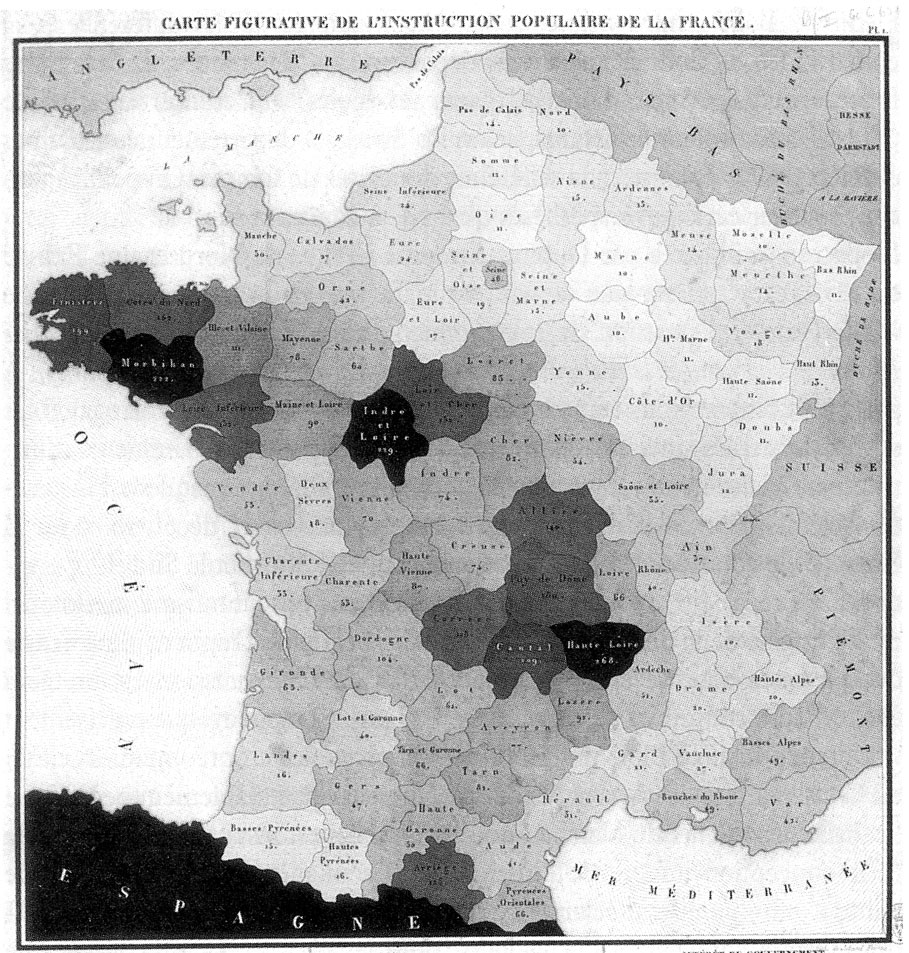
\includegraphics[width=0.4\textwidth]{analfabetismo-franca.jpg}
\caption{Mapa de Analfabetismo nas províncias francesas~\cite{mac}.}
\label{img:analfabetismo-franca}
\end{figure}


\section{Resultados}
\label{section:resultados}

De modo a avaliar a utilização da técnica de visualização computacional \textit{Choropleth Map}, foram realizados estudos de caso utilizando a base de dados do Atlas de Desenvolvimento Humano do PNUD Brasil do ano de 2013, contendo informações socioeconômicas de todos os estados e municípios brasileiros referentes aos anos de 1991, 2000 e 2010. Através da condução desses estudos, objetivou-se analisar algumas vantagens e restrições dessa técnica, assim como algumas análises do conjunto de dados.

\subsection{Comparativo do Índice de Educação}

Nesse primeiro estudo de caso, busca-se analisar a evolução dos dados de um indicador específico (índice de educação) em função do tempo através da comparação entre cada mapa.

Nas Figuras~\ref{img:educacao-1991},~\ref{img:educacao-2000} e~\ref{img:educacao-2010} estão apresentados o IDH-M Educação de cada município dos anos de 1991, 2000 e 2010; respectivamente. Torna-se perceptível a presença de índices inferiores (tonalidades mais escuras), de forma significativa, nas regiões Norte e Nordeste, assim como em diversos outros pontos. 

A partir do ano 2000, observa-se um crescimento no valor do indicador, principalmente nos estados do centro-sul. Por fim, no ano 2010, foi registrado um aumento significante em todo o país (tonalidades mais claras) de forma mais igualitária entre as regiões, ainda que inferior nas regiões Norte e Nordeste.

\begin{figure}[!ht]
\centering
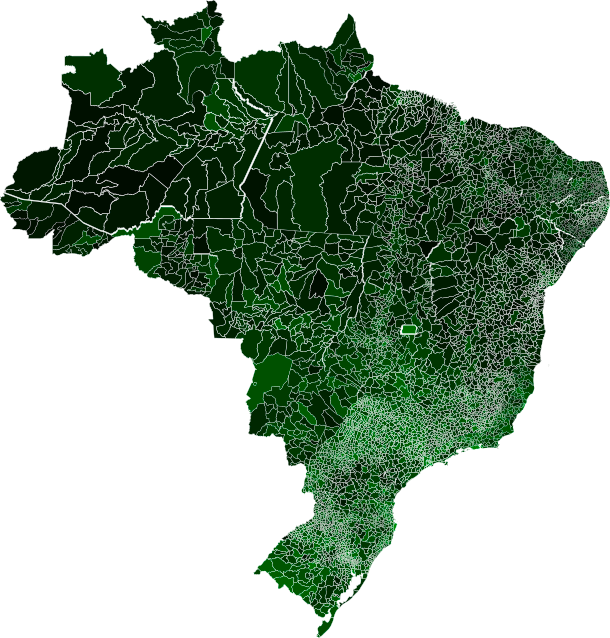
\includegraphics[width=0.40\textwidth]{educacao-1991.png}
\caption{IDH-M Educação no ano de 1991 (Fonte: Próprio autor).}
\label{img:educacao-1991}
\end{figure}

\begin{figure}[!ht]
\centering
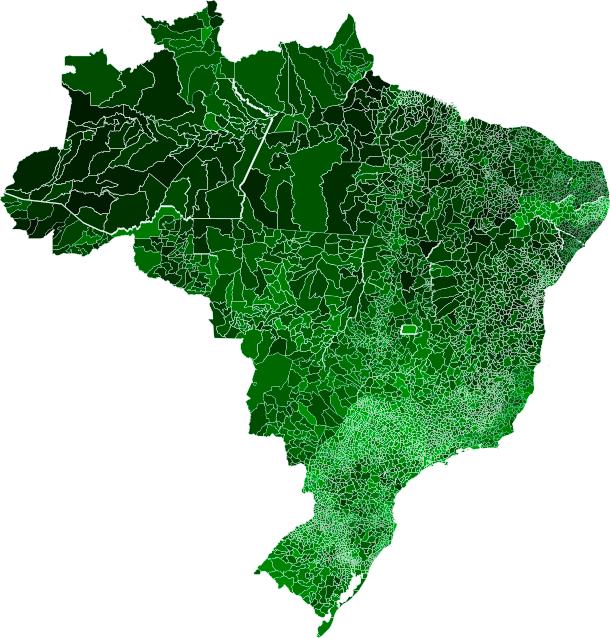
\includegraphics[width=0.40\textwidth]{educacao-2000.png}
\caption{IDH-M Educação no ano de 2000 (Fonte: Próprio autor).}
\label{img:educacao-2000}
\end{figure}

\begin{figure}[!ht]
\centering
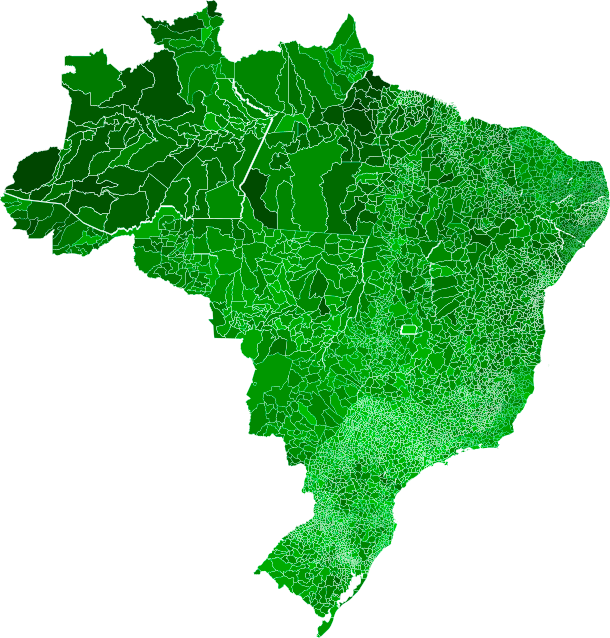
\includegraphics[width=0.40\textwidth]{educacao-2010.png}
\caption{IDH-M Educação no ano de 2010 (Fonte: Próprio autor).}
\label{img:educacao-2010}
\end{figure}


\subsection{Redimensionamento do Domínio de Dados}

\begin{figure}[!ht]
\centering
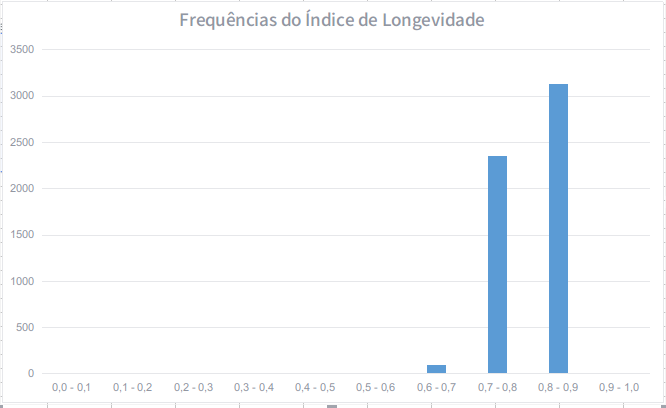
\includegraphics[width=0.40\textwidth]{frequencia.png}
\caption{Frequências do índice de longevidade (Fonte: Próprio autor).}
\label{img:histograma}
\end{figure}

\begin{figure}[!ht]
\centering
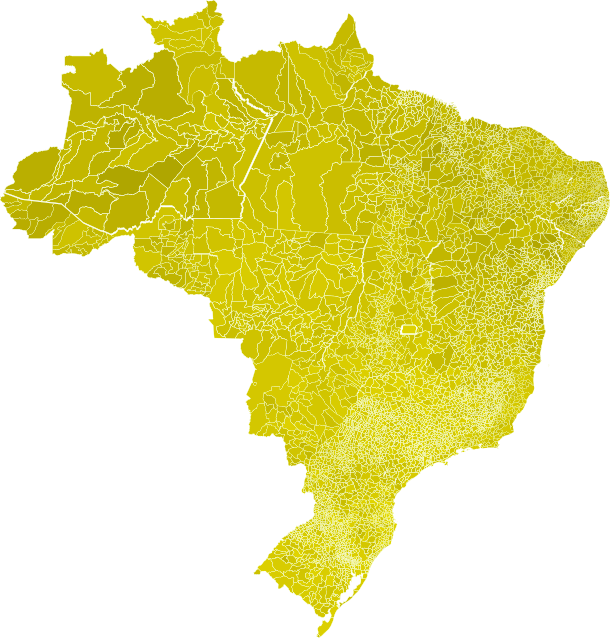
\includegraphics[width=0.40\textwidth]{longevidade.png}
\caption{Índice de Longevidade com os valores originais (Fonte: Próprio autor).}
\label{img:longevidade-absoluto}
\end{figure}

\begin{figure}[!ht]
\centering
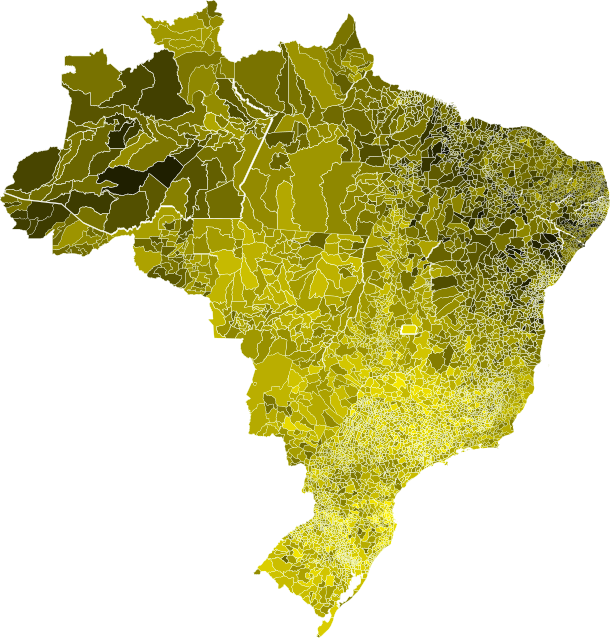
\includegraphics[width=0.40\textwidth]{longevidade-ampliado.png}
\caption{Índice de Longevidade com o domínio redimensionado (Fonte: Próprio autor).}
\label{img:longevidade-ampliado}
\end{figure}


\subsection{Evolução dos Índice de Desenvolvimento Humano}


\begin{figure}[!ht]
\centering
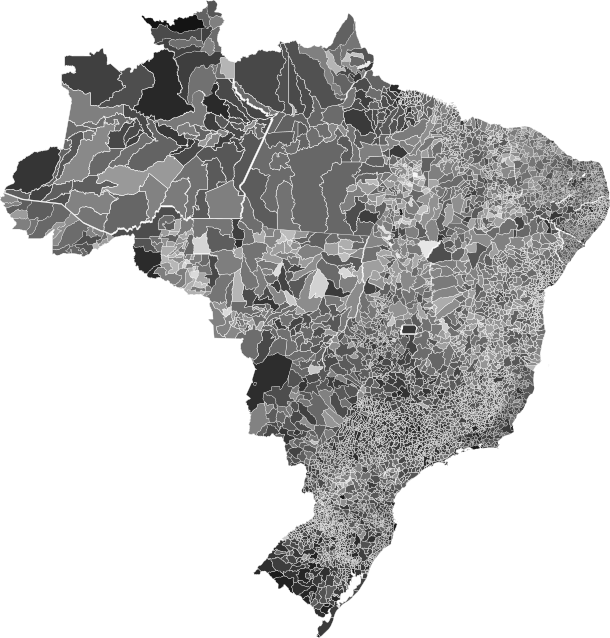
\includegraphics[width=0.40\textwidth]{evolucao.png}
\caption{Evolução do índice de desenvolvimento humano entre os anos de 1991 e 2010 (Fonte: Próprio autor).}
\label{img:evolucao-idh}
\end{figure}

\subsection{Qualidade de Vida no Brasil}

\begin{figure}[!ht]
\centering
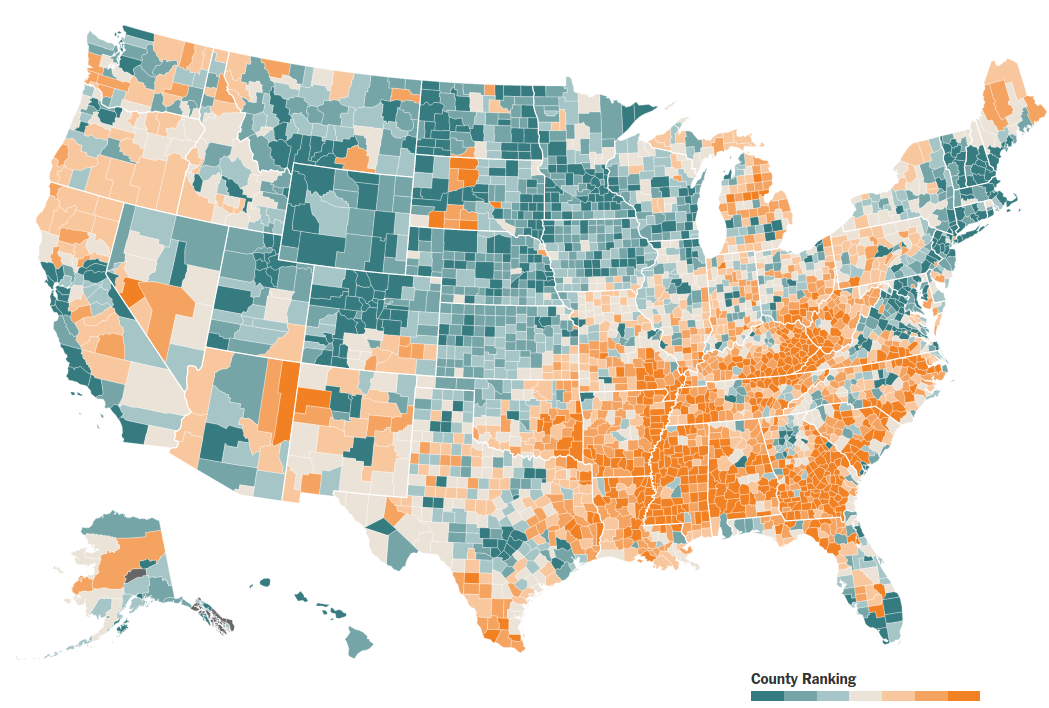
\includegraphics[width=0.40\textwidth]{usa.png}
\caption{Melhores lugares para se viver nos Estados Unidos~\cite{nytimes}.}
\label{img:lugares-viver-usa}
\end{figure}

\begin{figure}[!ht]
\centering
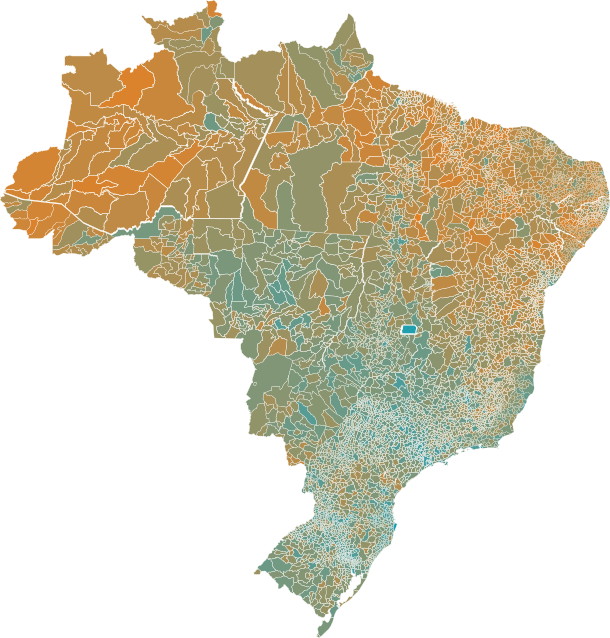
\includegraphics[width=0.40\textwidth]{qualidade-de-vida.png}
\caption{Qualidade de vida dos municípios do Brasil (Fonte: Próprio autor).}
\label{img:qualidade-de-vida-brasil}
\end{figure}

\section{Conclusão}
\label{section:conclusao}
The conclusion goes here.







\begin{thebibliography}{1}


\bibitem{atlas}
Programa das Nações Unidas para o Desenvolvimento (PNUD). \emph{Atlas do desenvolvimento humano do Brasil}. PNUD; 2003. Disponível em: http://www.pnud.org.br/atlas/

\bibitem{senak}
Sen AK. \emph{Desenvolvimento como liberdade}. São Paulo: Companhia das Letras; 2000.

\bibitem{espn}
Programa das Nações Unidas para o Desenvolvimento (PNUD). \emph{Informe sobre desarrollo humano: profundizar la democracia en un mundo fragmentado}. Espanha: Ediciones MundiPrensa; 2002.

\bibitem{oxford}
Programa das Nações Unidas para o Desenvolvimento (PNUD). \emph{Human development report: Millennium Development Goals: A compact among nations to end human poverty}. New York: Oxford University Press; 2003.

\bibitem{araujo}
Araujo PRM. \emph{Charles Taylor: para uma ética do reconhecimento}. São Paulo: Loyola; 2004

\bibitem{rezende}
Rezende, Amaury J. et al. \emph{A gestão pública municipal e a eficiência dos gastos públicos: uma investigação empírica entre as políticas públicas e o índice de desenvolvimento humano (IDH) dos municípios do Estado de São Paulo}. Revista Universo Contábil, 2005.

\bibitem{cesa}
Damásio, Bruno. \emph{Índice de Desenvolvimento Humano (IDH)}. Disponível em: <https://pascal.iseg.utl.pt/~cesa/index.php/dicionario-da-cooperacao/Glossary-1/\%C3\%8D/\%C3\%8Dndice-de-Desenvolvimento-Humano-\%28IDH\%29-261/>. Acesso em: 26 dez. 2017.

\bibitem{torguson}
Torguson, J. S. 2017. Choropleth Map. The International Encyclopedia of Geography. 1–9.

\bibitem{mac}
MacEachren, A M. Some Truth with Maps: a primer on symbolization \& design. Association of American Geographers. 1994.

\bibitem{nytimes}
Fippen, Alan. \emph{Where Are the Hardest Places to Live in the U.S.?}. Disponível em: <https://www.nytimes.com/2014/06/26/upshot/where-are-the-hardest-places-to-live-in-the-us.html>. Acesso em: 26 dez. 2017.

\end{thebibliography}




% that's all folks
\end{document}


